\chapter{Terraform}\label{sec:terraform}

Terraform è un Infrastructure as Code (IaC) tool, ovvero uno strumento che permette di definire infrastrutture cloud o on-premises tramite file di configurazione semplici da scrivere e da comprendere e che possono essere versionati, modificati e condivisi in base alle esigenze dell'utente. Tramite Terraform è possibile gestire sia componenti di basso livello (ad esempio server, reti, storage, ecc.) sia componenti di livello più alto, come ad esempio record DNS.

\section{Funzionamento}

Terraform crea e gestisce le risorse sulle piattaforme cloud o su altre piattaforme tramite le API fornite da tali servizi; purtroppo queste API non seguono uno standard e ogni provider implementa le proprie in maniera totalmente arbitraria, rendendo tendenzialmente difficile e dispendioso sviluppare tool che possano automatizzare le operazioni su più provider. Per questo motivo all'interno di Terraform esistono dei plugin, chiamati \emph{Terraform Provider} che hanno il compito di astrarre la connessione al provider (come mostrato in \cref{fig:terraform_how_works} e di fornire all'utente una serie di API di configurazione più o meno standard. Esistono migliaia di provider sviluppati sia dalla community che da HashiCorp (l'azienda madre di Terraform); tra questi sono presenti anche quelli che permettono l'interfacciamento con le piattaforme cloud più utilizzate (AWS, GCP, Azure, ...). È possibile cercare e consultare la documentazione di tutti i provider sul \emph{Terraform Registry}\footnote{Terraform Registry: \url{https://registry.terraform.io}}.

\begin{figure}[H]
    \center
    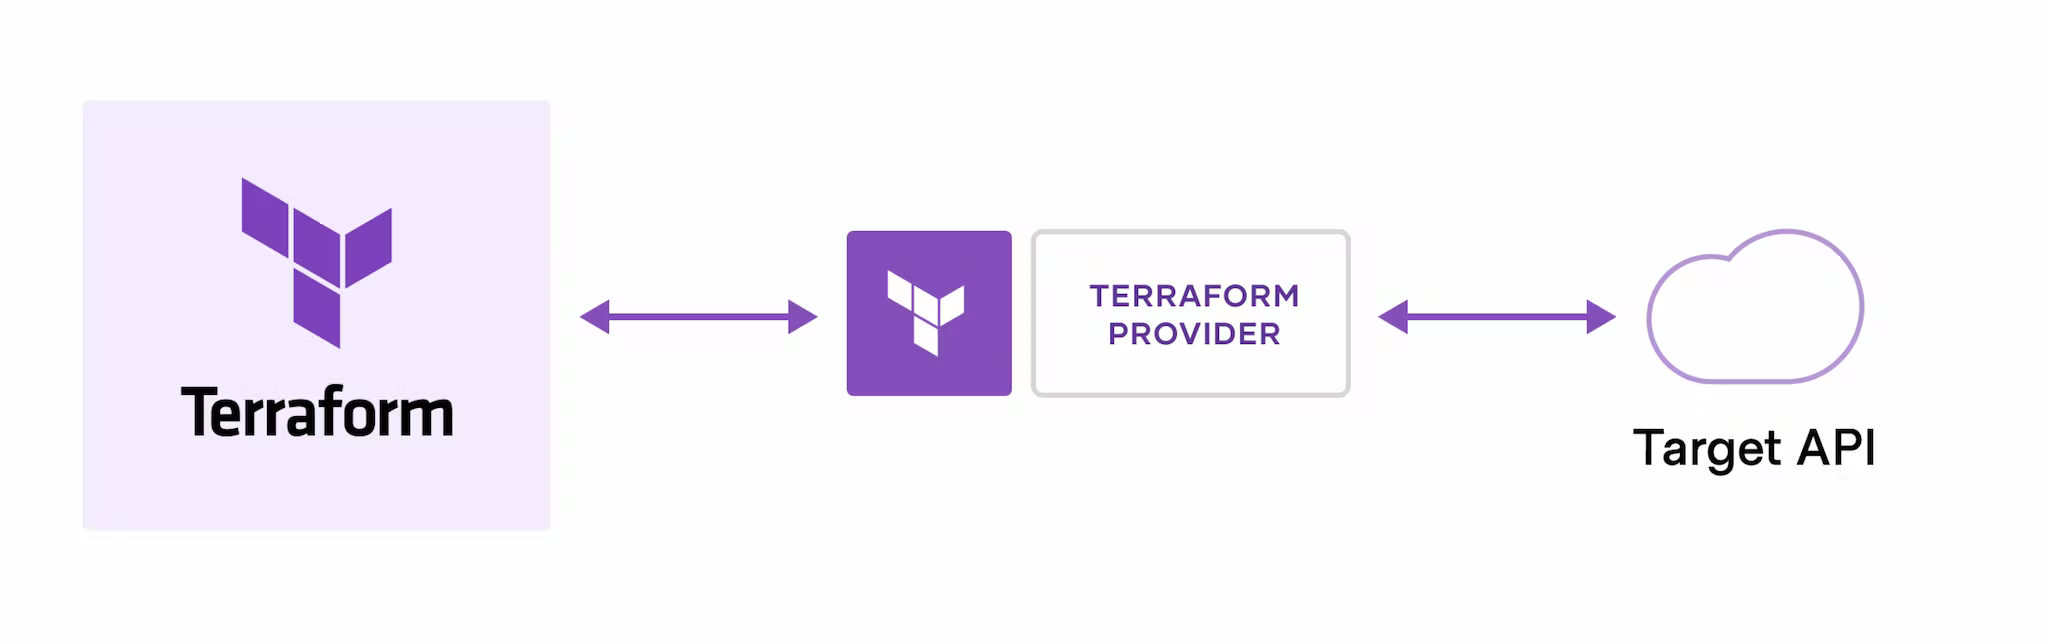
\includegraphics[scale=0.1]{tesi/files/immagini/terraform/how_works.png}
    \caption{Schema di funzionamento di Terraform}
    \label{fig:terraform_how_works}
\end{figure}

\section{Utilizzo}

\subsection{Workflow}

L'utilizzo di Terraform modifica notevolmente il workflow di chi deve progettare e realizzare un'infrastruttura cloud riducendo sensibilmente i tempi richiesti per la configurazione dell'infrastruttura stessa e per la manutenzione. Il workflow con Terraform è composto infatti da 3 step (come mostrato in \cref{fig:terraform_workflow}):
\begin{itemize}
    \item \textbf{Write}: si definisce l'infrastruttura desiderata tramite i file di configurazione di Terraform; questa infrastruttura può includere anche provider multipli
    \item \textbf{Plan}: Terraform individua quali elementi della configurazione fornita devono essere creati o distrutti; questa decisione viene presa in base alla configurazione e alle risorse dell'infrastruttura già esistente
    \item \textbf{Apply}: una volta che l'utente ha approvato le modifiche proposte, Terraform esegue le operazioni di aggiornamento creando e/o distruggendo risorse
\end{itemize}

\begin{figure}[H]
    \center
    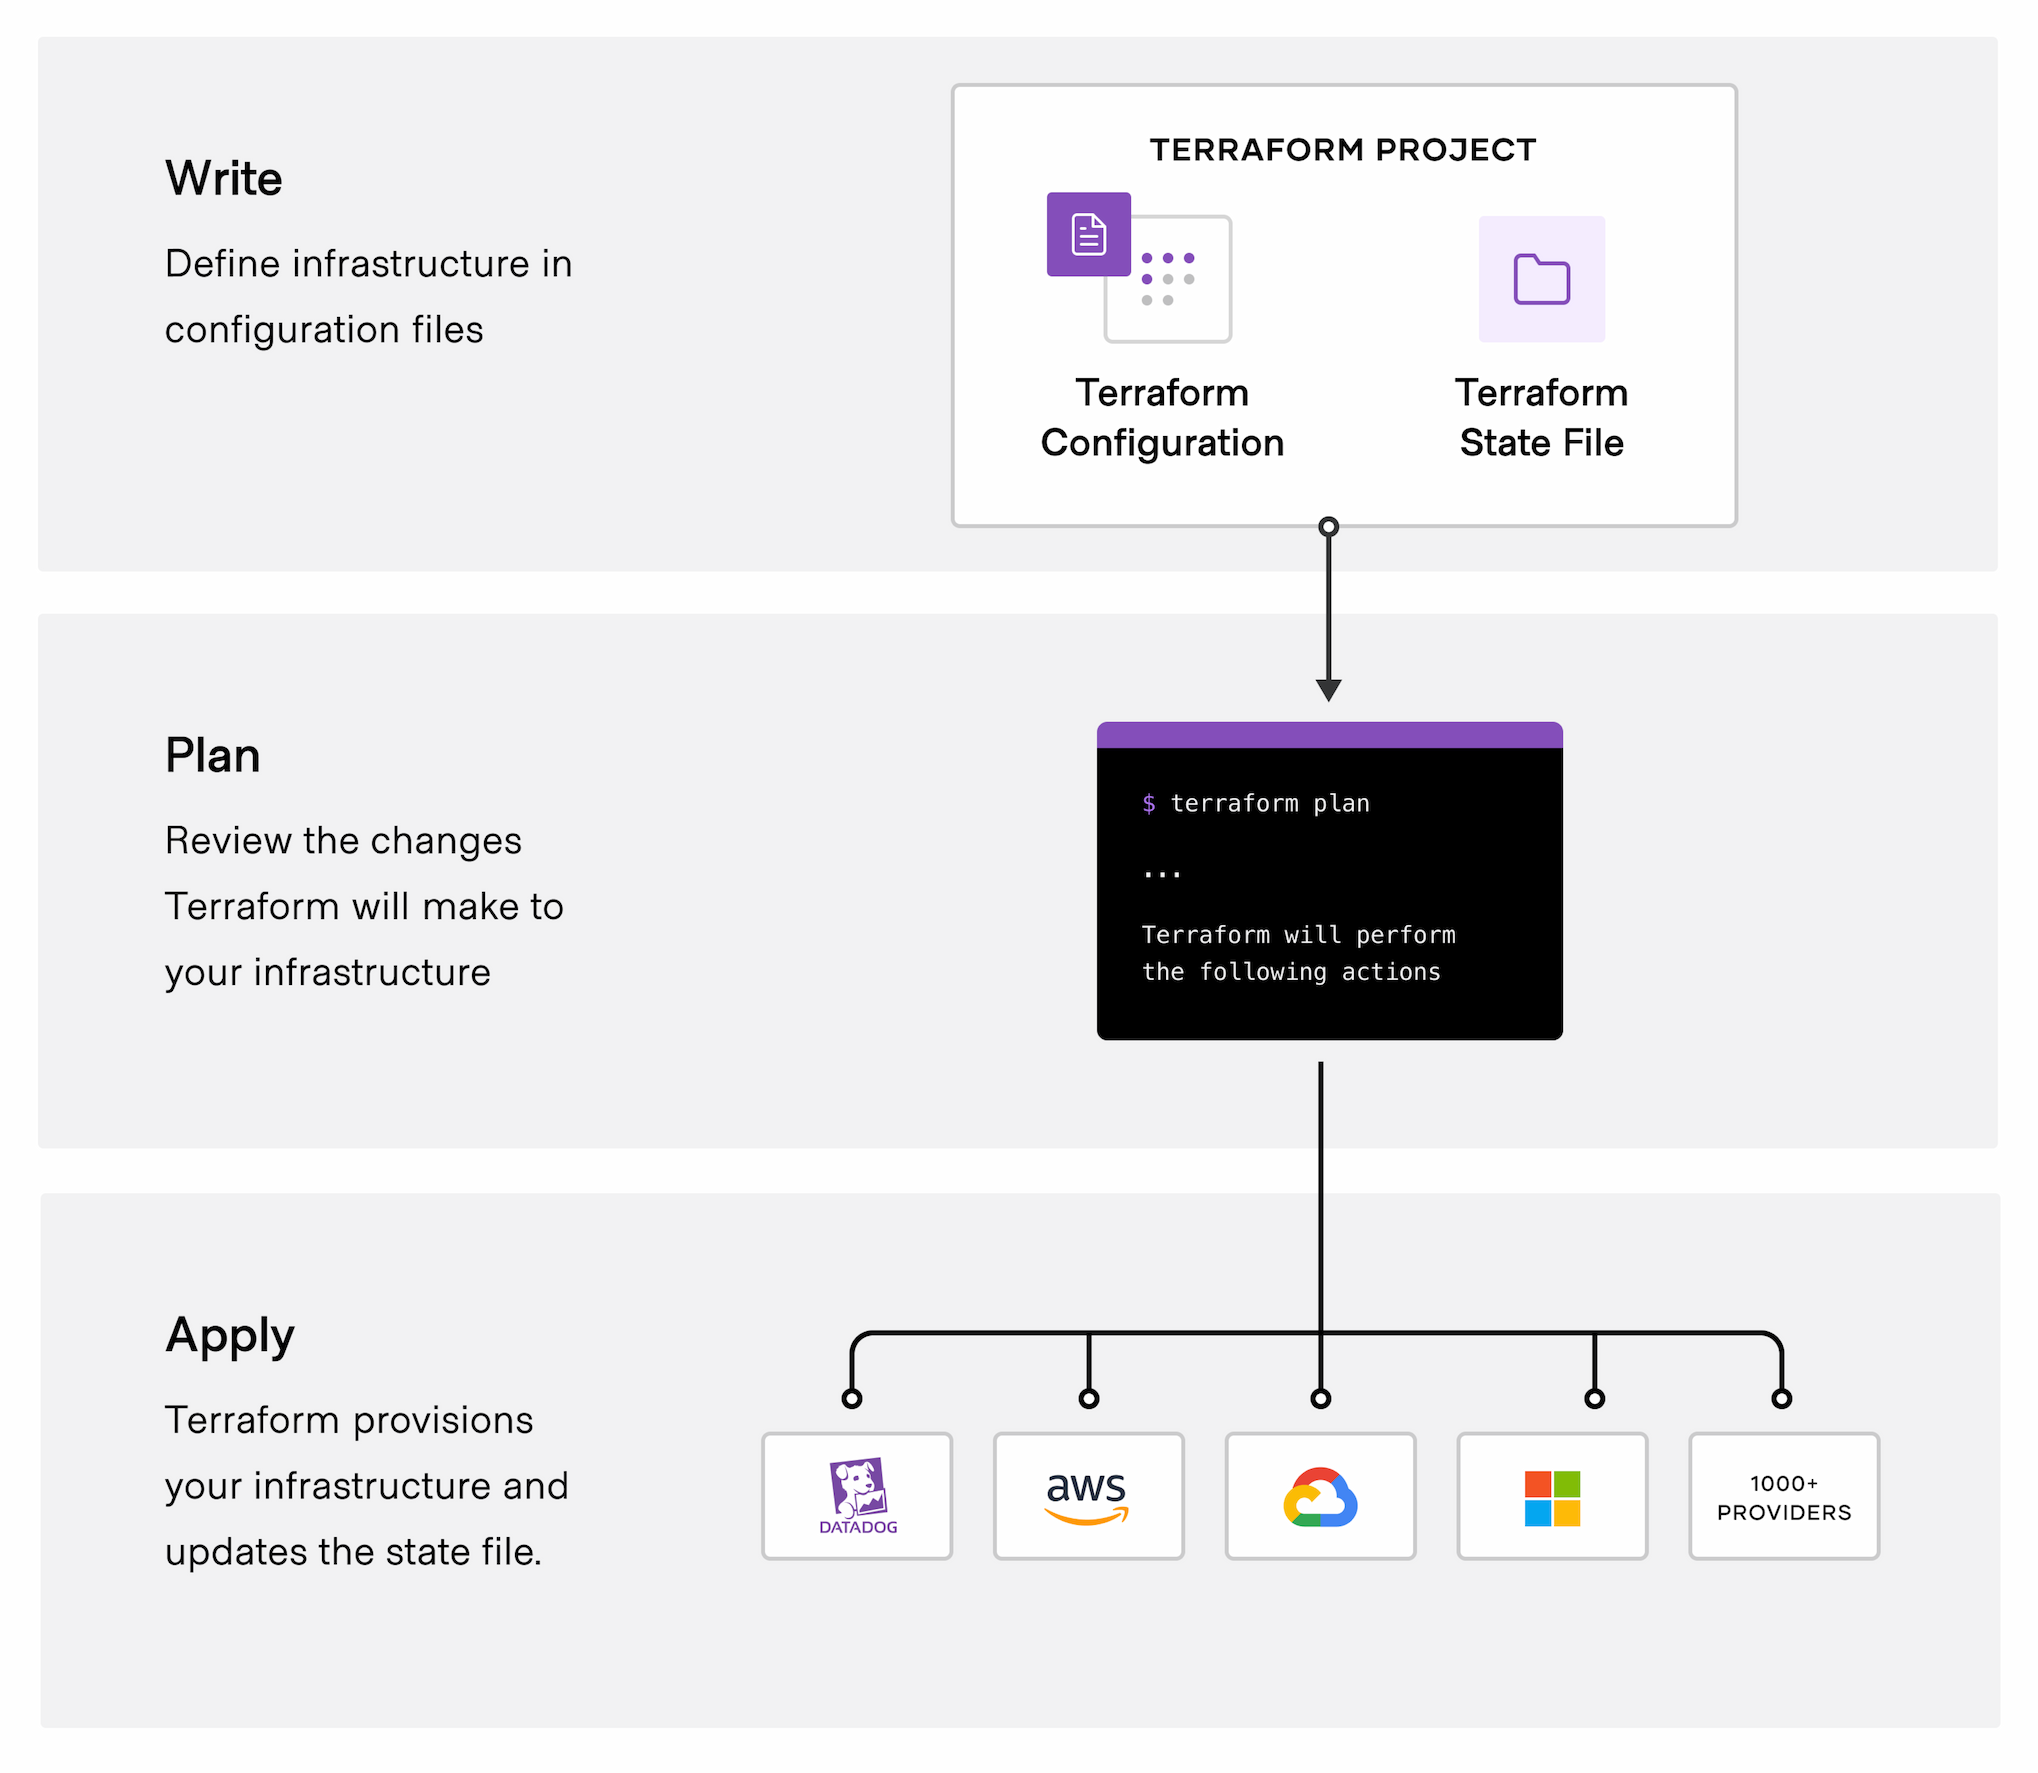
\includegraphics[scale=0.15]{tesi/files/immagini/terraform/workflow.png}
    \caption{Workflow con Terraform}
    \label{fig:terraform_workflow}
\end{figure}

\subsection{Progetti con Terraform}

Un progetto Terraform è la configurazione di un'infrastruttura che si vuole modellare; questa infrastruttura può appoggiarsi su più provider e quindi essere distribuita su più cloud. I progetti Terraform possono assumere diverse strutture più o meno complesse e generalmente tale struttura varia in base alla complessità dell'infrastruttura da definire.

Per un progetto molto semplice è sufficiente creare una cartella all'interno della quale si scrive il file \verb|main.tf| che contiene la configurazione dell'infrastruttura che volgiamo realizzare. Ogni volta che si crea un nuovo progetto o si aggiungono provider ad uno esistente è necessario eseguire il comando \verb|terraform init| in modo che vengano scaricati i provider necessari al progetto.

Una volta terminata la configurazione si possono verificare le modifiche eseguite lanciando il comando \verb|terraform plan|; l'output mostrerà tutte le operazioni che Terraform intende eseguire per applicare la configurazione definita partendo dalle risorse già esistenti. Per applicare le modifiche si deve lanciare il comando \verb|terraform apply| che, dopo aver mostrato nuovamente le operazioni che intende eseguire, chiederà una conferma all'utente e poi procederà con l'aggiornamento dell'infrastruttura.

Se si vuole cancellare completamente tutta l'infrastruttura creata è sufficiente lanciare il comando \verb|terraform destroy| che, dopo aver chiesto conferma all'utente, cancellerà tutte le risorse associate al progetto.

\subsection{Configurazioni di Terraform: HCL}

HCL (HashiCorp Configuration Language) è un toolkit sviluppato direttamente da HashiCorp che permette di creare linguaggi di configurazione strutturati che siano facilmente comprensibili dagli essere umani e al contempo facilmente interpretabili dalle macchine. HCL supporta sia una sintassi nativa che il formato JSON (tendenzialmente utilizzato quando i file di configurazione vengono generati automaticamente). Tutti i file di configurazione di Terraform utilizzano una sintassi basata su HCL.

\paragraph{Argomenti e Blocchi.}

Il linguaggio di Terraform si basa su due elementi principali: argomenti e blocchi.
Gli argomenti sono l'equivalente delle variabili in un linguaggio di programmazione tradizionale, ovvero permettono di associare un valore ad un nome definito dall'utente, come nell'esempio seguente:
\begin{lstlisting}[language=hcl]
image_id = "abc123"
\end{lstlisting}

I blocchi sono invece contenitori per altro contenuto; ciascun blocco è definito da un tipo e, in base ad esso, cambia il numero di etichette da inserire dopo la definizione del tipo del blocco. Nell'esempio che segue è definito un blocco di tipo \verb|resource| che accetta 2 etichette (in questo caso \verb|"aws_instance"| e \verb|"example"|):
\begin{lstlisting}[language=hcl]
resource "aws_instance" "example" {
    ...
}
\end{lstlisting}

\paragraph{Espressioni condizionali.}

Le espressioni condizionali permettono di selezionare uno tra due valori utilizzando un'espressione booleana; la sintassi di queste espressioni è la seguente:
\begin{lstlisting}[language=hcl]
condition ? true_val : false_val
\end{lstlisting}
Gli operatori logici e di comparazione utilizzabili all'interno della condizione sono analoghi a quelli utilizzabili nel linguaggio C (\verb|==|, \verb|!=|, \verb|<=|, \verb|&&|, \verb|!|, ...)

\paragraph{Espressioni iterative.}

All'interno del linguaggio di Terraform è integrata l'espressione \verb|for| che, analogamente all'omonimo costrutto dei linguaggi di programmazione, serve per eseguire delle iterazioni. Tramite l'utilizzo di questa espressione è possibile iterare sia le liste che le mappe; di seguito sono riportati due esempi:
\begin{lstlisting}[language=hcl]
# iterazione di una lista
[for s in var.list : upper(s)]
# iterazione di una mappa
[for k, v in var.map : length(k) + length(v)]
\end{lstlisting}

\paragraph{Blocchi dinamici.}

I blocchi dinamici agiscono in maniera simile alle espressioni \verb|for|, con la differenza che l'output è un insieme di blocchi. Questo tipo di blocco può essere usato solamente all'interno di altri blocchi e, nello specifico, all'interno di blocchi di tipo \verb|resource|, \verb|data|, \verb|provider| o \verb|provisioner|. Di seguito è riportato un esempio di configurazione contenente un blocco dinamico:
\begin{lstlisting}[language=hcl]
resource "aws_elastic_beanstalk_environment" "tfenvtest" {
  name                = "tf-test-name"
  application         = "${aws_elastic_beanstalk_application.tftest.name}"
  solution_stack_name = "64bit Amazon Linux 2018.03 v2.11.4 running Go 1.12.6"

  dynamic "setting" {
    for_each = var.settings
    content {
      namespace = setting.value["namespace"]
      name = setting.value["name"]
      value = setting.value["value"]
    }
  }
}
\end{lstlisting}
In questo caso l'etichetta \verb|"setting"| indica il tipo di blocco, l'argomento \verb|for_each| indica i valori che devono essere iterati per la generazione dei blocchi e il blocco \verb|content| definisce quale deve essere la struttura dei blocchi generati.